\documentclass[a4paper]{ltjsarticle}

\usepackage{amsmath} % 数式を記述するためのパッケージ
\usepackage{graphicx} % 画像を挿入するためのパッケージ
\usepackage{url} % URLを記述するためのパッケージ
\usepackage{here} % 図表をその場所に表示するためのパッケージ
\usepackage{luacode} % ソースコードを記述するためのパッケージ
\usepackage{titling} % タイトルをカスタマイズするためのパッケージ
\usepackage{fancyhdr} % ヘッダーをカスタマイズするためのパッケージ
\usepackage{siunitx}
\usepackage{multirow}
\usepackage{bigdelim}
\usepackage{amssymb}
\usepackage{listings}
\usepackage{xcolor}
\usepackage{multicol}
\usepackage[subrefformat=parens]{subcaption}

\definecolor{codegreen}{rgb}{0,0.6,0}
\definecolor{codegray}{rgb}{0.5,0.5,0.5}
\definecolor{codepurple}{rgb}{0.58,0,0.82}
\definecolor{backcolour}{rgb}{0.95,0.95,0.92}

\lstdefinestyle{mystyle}{
    backgroundcolor=\color{backcolour},   
    commentstyle=\color{codegreen},
    keywordstyle=\color{blue},
    numberstyle=\tiny\color{codegray},
    stringstyle=\color{codepurple},
    basicstyle=\ttfamily\footnotesize,
    breakatwhitespace=false,         
    breaklines=true,                 
    captionpos=b,                    
    keepspaces=true,                 
    numbers=left,                    
    numbersep=5pt,                  
    showspaces=false,                
    showstringspaces=false,
    showtabs=false,                  
    tabsize=2,
    title=\lstname
}
\lstset{style=mystyle}


\preauthor{\begin{flushright}} % authorを右寄せにする
\postauthor{\end{flushright}}
\predate{\begin{flushright}} % dateを右寄せにする
\postdate{\end{flushright}}

\pagestyle{fancy}
\lhead{電気電子情報実験・演習第一 I3実験レポート}
\rhead{03240403 井上聡士}
\cfoot{\thepage}
\renewcommand{\headrulewidth}{0pt}


\title{電気電子情報実験・演習第一 I3実験レポート}
\author{電子情報工学科 \\ 03240403 井上聡士}
\date{2024年6月28日}


\begin{document}
\maketitle % タイトルページを表示する
\section{目標}
普通の通話アプリ(Zoom、Skype等)には、以下のような機能が存在する
\begin{itemize}
    \item 音声通話
    \item 多人数通話
    \item マイクのミュート
    \item カメラのオン・オフ
    \item 画面共有
    \item チャット
\end{itemize}
このうち、カメラ関係の機能は、WSL2においてカメラのインターフェイスがどうなっているのかわからないことにより断念した。
そのため、I3課題では以下の機能を実装することを目標とした。
\begin{itemize}
    \item 多人数通話
    \item ニックネームの設定
    \item マイクのミュート・アンミュート
    \item チャット
\end{itemize}

\section{多人数通話}
多人数通話をするにあたって、問題点が4点存在する。
\begin{itemize}
    \item そもそもどのように通信を行うか
    \item 単位時間に送信するデータ量と受信するデータ量が大きく異なり、人数に依存する中どのようにデータの送受信を行うか
    \item 音声、チャット等様々なデータをどう区別するか
    \item 受信した音声をどのように再生すれば重ねることが出来るか
\end{itemize}

\subsection{通信方式}
\begin{figure}[htbp]
    \centering
    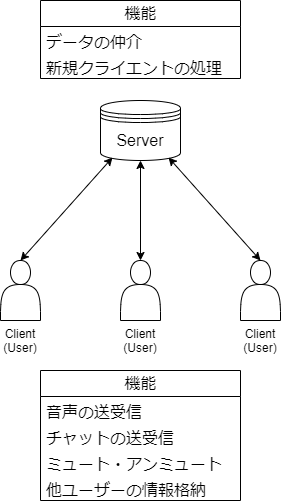
\includegraphics[width=0.8\columnwidth]{./images/server_client.png}
    \caption{通信方式の設計と機能}
    \label{fig:server_client}
\end{figure}
そもそも基本的にサーバー・クライエントは1対1で通信を行うため、多人数通話を行うにはサーバー・クライエントの通信を複数行う必要がある。
ただし、クライエント(=アプリのユーザー)が複数の他のクライエントに接続するのは、非常に難しく、そもそも通信に負荷がかかるうえ、さらにクライエント同士で接続する際にどちらがサーバーとなるかわからないという問題も存在する。
そのため、サーバー側で複数のクライエントを処理し、それぞれのクライエントに複数のクライエント分のデータを送ることで、多人数通話を実現することにした(図\ref{fig:server_client})。
サーバーは基本的にデータの仲介のみを行い、それ以外の機能を担わないが、例外として新しいクライエントが接続してきたときに他のクライエントの現在の状況(ニックネーム、ミュート状態)を送る。
クライエントで多くの処理を行い、音声、ミュート・アンミュート、チャットの情報を受け取った後にそれを処理する。

さて、既存のクライエントや新しい接続を試みるクライエントが存在するとき、どのように処理するべきか。
通常の\verb|recv|関数は、基本的に相手から信号を受信するまで待機し続け、その間に他の処理を実行することが出来ない。
そこで、\verb|select|という関数を使用した。
\verb|select|関数は、複数のfile descriptorに対して、読み込み、書き込み、例外のいずれかが発生するまで待機する関数であり、逆にいえばどれか一つが変化すれば処理を行うことが出来る。
基本的な使用方法は、以下の通りである。
\begin{lstlisting}[language=C]
fd_set readfds;
int maxfd = 0;
while (1) {
    FD_ZERO(&readfds); // readfdsを初期化
    FD_SET(fd0, &readfds); // 全てのfile descriptorをreadfdsに追加
    ...
    FD_SET(fdN, &readfds);
    maxfd = max(maxfd, fd0, fd1, ..., fdN); // 最大のfile descriptorを取得
    select(maxfd + 1, &readfds, NULL, NULL, NULL); // いずれかのfile descriptorが変化するまで待機
    if (FD_ISSET(fd0, &readfds)) {
        // fd0に変化があった場合の処理
    }
    ...
    if (FD_ISSET(fdN, &readfds)) {
        // fdNに変化があった場合の処理
    }
}
\end{lstlisting}
実際のサーバーのスクリプトでは、新規クライエントからの接続はサーバーの\verb|socket|の変化を、既存のクライエントからのデータは各クライエントの\verb|socket|の変化を検知することで処理した。

\subsection{クライエント側のデータ処理}
クライエント側は、通話に参加しているユーザーの数により受信するデータ量が変化するため、I2で行ったようにデータを受信・送信交互に行っても遅延が生じてしまう。
そのため、ノンブロッキングモードで入力した音声データの送信と受信したサーバーデータの処理を行う必要がある。

この処理も、\verb|select|関数を使用して行った。\verb|connect|したサーバーの\verb|socket|と、起動した\verb|sox|の\verb|socket|(および後述するが標準入力\verb|stdin|の\verb|socket|である\verb|STDIN_FILENO|)を\verb|select|関数に登録し、どちらかに変化があった場合に処理するようにした。

\subsection{データの区別}
サーバーからは、自分以外のクライエント分の音声データ、チャットデータ、及びクライエントの状態(ミュート・アンミュート、ニックネーム)変化のデータが送られてくるが、これを区別する必要がある。
そこで、サーバーへの送信データおよびサーバーからの受信データの先頭に、クライエント番号とデータの種類を示す識別番号を付与することで、クライエント側でデータの種類を判別することにした。
サーバーへ送信するときは、識別番号をそれぞれ以下の通りに設定した
\begin{itemize}
    \item 1: マイクからの音声データ
    \item 2: チャットのデータ
    \item 3: ミュート・アンミュートのデータ
    \item 4: ニックネーム・表示名のデータ
\end{itemize}
サーバーから受信するときは、識別番号をそれぞれ以下の通りに設定した。
\begin{itemize}
    \item 0: サーバーからのメッセージ(主にサーバーへの接続で帰ってくるメッセージ)
    \item 1: 新規クライエントの接続・通話への参加
    \item 2: 他のクライエントの切断・通話からの離脱
    \item 3: 音声データ
    \item 4: チャットのデータ
    \item 5: ミュート・アンミュートの変更
    \item 6: ニックネーム・表示名の変更
\end{itemize}
そして、各TCPパケットの先頭に、サーバーへの送信データは\verb|(識別番号)>>|を、サーバーからの受信データは\verb|(クライエント番号).(識別番号)>>|をつけて送信した。

しかし、ここで3つほど問題点が浮上した。
\begin{itemize}
    \item 付けた修飾子\verb|...>>|の文字数が不定で、どこまで読み取ればいいのか不明である
    \item 修飾子\verb|...>>|が音声データやチャットデータにも含まれてしまうと、音声データが途中で切れたりしてしまい、挙動が不安定になる
    \item \verb|recv|で特定の文字数を取得しようとしても、それより短い文字数しか取得できない場合がある
\end{itemize}
上の二つは、どちらも「\verb|recv|する文字数が不明である」という共通の問題点に起因している。
これを解決するために、まず、修飾子\verb|...>>|の文字数を統一した。接続するクライエントは最大30に設定してあったため、クライエント番号を2桁表記\verb|%02d|にすることで解決した。
次に、2番目の問題だが、これは事前に読み取るデータの長さを指定することで回避できる。音声データは1024バイトずつ送信することに決めていたので、1回のパケットで送る最大データ量を1024バイト+修飾子として、その送信するデータ量を修飾子の中に記述した。
例えば、140バイトの文字列をサーバーへ送信する場合、\verb|2.0140>>|と記述した後に140字の文字列を送信することで、サーバー側で140バイトの文字列として処理でき、仮に\verb|2.0300>>|などの文字列がデータ中に現れても問題なく文字として処理できる。

最後に、3番目の問題は、検証した結果、TCPパケットをすべて受信できる前に\verb|recv|を呼び出したことによるものだと判明した。
通常TCPパケットはデータ量が大きいと何回かに分割して送るが、そのうち一つしか受信できてないうちに\verb|recv|を呼ぶと意図していたよりも短いデータしか読み取れない。
これを修正するために、パケットのすべてのデータを受け取るまで待つ\verb|recv_all|という関数を定義した。

\subsection{音声の入力・出力}
音声の入力・出力には、\verb|sox|を使用した。
ただし、チャット機能を実装するが故、標準入力は必要であったので、\verb|popen|を使用して独自のfile descriptorから入力を取ることで、\verb|sox|と標準入力を同時に行うことが出来るようにした。

出力は、これより難易度が高かった。
\verb|sox|のマニュアルを見ると、複数の入力を同時に再生することが可能で、かつ\verb|-v|をつけることでそれぞれの入力の音量を独自に調整できるようなので、これを試みた\cite{sox manual}。
そこで、クライエント側で、他の各クライエントの音声入力を収納する一時ファイル\verb|tmp01.tmp|、\dots\verb|tmpN.tmp|を作成し、それを
\begin{lstlisting}[language=bash]
    $ sox -m -q -t s16 -r 44100 -c 1 tmp01.tmp -t s16 -r 33100 -c 1 tmp02.tmp ... -d
\end{lstlisting}
として、\verb|popen|で実行するようにした。また、新しいクライエントが入ったときは元の\verb|popen|を\verb|pclose|で閉じて、新しいものを開くようにした。
しかし、これはうまく動作しなかった。音声は重なったが、一定の時間再生された後再生されなくなった。
これは、\verb|sox|が、起動された時までの\verb|.tmp|ファイルの分の時間しか再生しなかったためであると考えられる。

そこで、この解決策、すなわち\verb|popen|を起動した後のファイルの更新を読み取る仕組みを考えた。
このとき、2通りの似たような方法にたどり着いた。

一つ目は、\verb|tail -f|コマンドによる追跡である\cite{tail command}。\verb|tail -f|コマンドは、あるファイルを追跡し、随時更新されるたびに新たな出力を生み出し、かつキャンセルされるまで終了しない関数である。
\verb|sox|コマンドは、パイプのような形で複数のコマンド出力を取ることも可能であり、以下のように記述される。
\begin{lstlisting}[language=bash]
    $ sox -m -q -t s16 -r 44100 -c 1 "|tail -f tmp01.tmp" -t s16 ...
\end{lstlisting}
これを\verb|popen|で実行することで、\verb|sox|が\verb|tmp01.tmp|、\verb|tmp02.tmp|、...の更新を追跡し、新たな音声データが追加されるたびに再生することが出来る。
しかし、新たなクライエントが登場し、\verb|pclose|でこのコマンドを閉じようとしても閉じず、そこでフリーズするという問題点が発生した。
これは、\verb|pclose|の特性上、実行しているプログラムを\verb|kill|のように強制終了するのではなく、終了するまで待つためである。
しかし、\verb|sox|によりパイプされた\verb|tail -f|は、おそらくサブプロセスとして実行され、\verb|sox|が終了しても\verb|tail -f|は終了しないため、\verb|pclose|が終了しないと考えられる。

二つ目は、\verb|FIFO|(First in, first out)という種類のファイルを使用することである。
\verb|FIFO|は、ファイルシステム上に存在するファイルであり、書き込まれたデータは読み取られるまで保持される\cite{fifo command}。
外見上は他の普通のファイルと変わりはないが、\verb|ls -l|コマンドで\verb|p|という文字が先頭についていることで\verb|FIFO|であることがわかる。
\verb|FIFO|は、\verb|mkfifo|コマンドで作成することが出来る。
また、この\verb|FIFO|は、ファイルの書き込みと読み込みを同時に開く必要があり、同時開かれるまで\verb|open|の行で止まったままになってしまう。
そのため、\verb|open|を別スレッドで行うことで、\verb|FIFO|を開こうとした。
\verb|fork|関数を使用して、まず親プロセスで\verb|sox|を起動し、子プロセスで\verb|FIFO|(読み取り)を開き、その後親プロセスで\verb|open|(書き込み)をすることで、\verb|FIFO|を同時に開くことが出来た。
しかし、これもうまく動作しなかった。
検証を重ねていくうちに、おそらく\verb|sox|コマンドが複数の\verb|FIFO|の入力に対応していないことが判明した。

そのため、最終的には、一つの\verb|sox|コマンドですべてのクライエントの音声を再生することは不可能であると判断した。
そこで、複数の\verb|sox|コマンドを起動し、それぞれのクライエントの音声を再生することにした。

この方針は簡単で、\verb|popen|により複数のコマンドを同時に起動し、それぞれの入力file descriptorに書き込むことで実現できた。

\section{チャット}
チャットはいたって簡単である。
クライエント側の\verb|select|で、標準入力も監視し、変更があった際に識別子を付けてサーバーに送信する。
受信する際は、読み取った識別子からチャットであることを判断し、それを標準出力に出力する。

\section{コマンド}
ミュート・アンミュート、および名前の変更は、標準入力で\verb|/mute|、\verb|/unmute|、\verb|/name <名前>|と入力することで行うことが出来る。
標準入力のデータを、\verb|strncmp|で比較し、最初の文字が\verb|/|であればコマンドと認識し、それ以降の文字列を処理する。

ミュートをしたときには、音声データを単に送信しないようにした。

\section{コード}
\subsection{実行}
コンパイルしたサーバー側のファイルを以下のように実行する。
\begin{lstlisting}[language=bash]
$ ./multi_server <ポート番号>
\end{lstlisting}
別のターミナルで、コンパイルしたクライエント側のファイルを以下のように実行する。
\begin{lstlisting}[language=bash]
    $ ./multi_client <サーバーのIPアドレス> <ポート番号>
\end{lstlisting}

\subsection{実演}
レポートを書く際は4つのターミナルを用意し、サーバーを起動した後3つのクライエントを起動した。
尚、別のPCで実行しても動作することは確認済みである。
\begin{figure}[htbp]
    \centering
    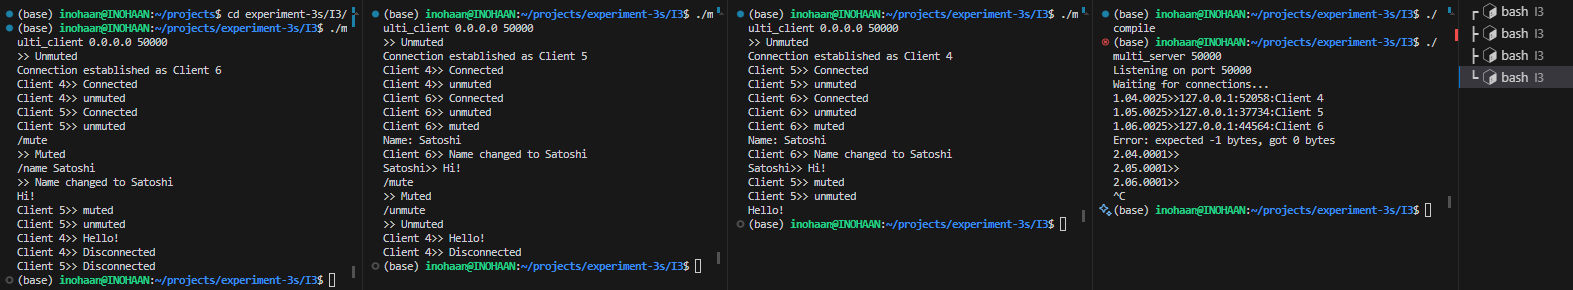
\includegraphics[width=0.98\columnwidth]{./images/terminal_show.png}
    \caption{実演した際の様子}
    \label{fig:terminal_show}
\end{figure}
図\ref{fig:terminal_show}は、この時の様子である。
サーバーを起動した後、左側のクライエントから順に起動した。
新しいクライエント(左から2つめの\verb|Client 5|)が参加すると、既存の\verb|Client 4|には\verb|Client 5>> Connected|と表示され、接続されたことが表示される。
また、参加した\verb|Client 5|も、すでにいる\verb|Client 4|の情報を受け取っている。

最後に参加した\verb|Client 6|が\verb|/mute|コマンドを使用すると、\verb|Client 6>> muted|と表示され、\verb|Client 6|の音声が送信されなくなる。
また、\verb|name Satoshi|とした後は、\verb|Client 6>>|の代わりに\verb|Satoshi>>|と表示されている。
\verb|Hi!|と入力すると他のクライエントにも\verb|Satoshi>> Hi!|と表示されているように、チャットも機能している。

また、クライエントが切断すると、\verb|Client 4>> Disconnected|のように、切断も表示される。

レポートで紹介した機能は正常に動作しているだろう。

\subsection{サーバー側のコード}
\begin{multicols}{2}
    \lstinputlisting[language=C]{multi_server.c}
\end{multicols}
\subsection{クライエント側のコード}
\begin{multicols}{2}
    \lstinputlisting[language=C, title=multi\_client.c]{multi_client_new.c}
\end{multicols}

\begin{thebibliography}{99}
    \bibitem{sox manual} Bagwell, C. (n.d.). sox(1) - Linux man page. die.net. Retrieved June 29, 2024, from \url{https://linux.die.net/man/1/sox}
    \bibitem{tail command} GeeksforGeeks. (2023, December 13). Tail command in Linux with examples. GeeksforGeeks. \url{https://www.geeksforgeeks.org/tail-command-linux-examples/}
    \bibitem{pclose manual} pclose(3) - Linux man page. (n.d.). die.net. Retrieved June 30, 2024, from \url{https://linux.die.net/man/3/pclose}
    \bibitem{fifo command} GeeksforGeeks. (2023, September 9). Named Pipe or FIFO with example C program. GeeksforGeeks. \url{https://www.geeksforgeeks.org/named-pipe-fifo-example-c-program/}
\end{thebibliography}

\end{document}